\documentclass[12pt]{standalone}

\RequirePackage{times}
\RequirePackage{amsmath}
\RequirePackage{amssymb}
\RequirePackage[T1]{fontenc}

\usepackage{tikz}
\usepackage{xcolor}
\usepackage{pgfplots}
\pgfplotsset{compat=1.16}
\usetikzlibrary{backgrounds,calc,positioning}

\definecolor{red}{HTML}{972e21}
\definecolor{yellow}{HTML}{ebb83f}
\definecolor{blue}{HTML}{7999db}

\begin{document}
	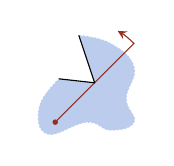
\begin{tikzpicture}[x=1cm,y=1cm]
		\path (-0.35,-0.2) rectangle (1.15,1.2);
		\newcommand{\contour}{(0.05,0.55) (-0.2,0.2) (-0.1,-0.15) (0.4,0) (0.7,-0.1) (1,0) (0.9,0.3) (1,0.7) (0.7,1) (0.3,1.1)}
		\draw[blue!50,line cap=round,densely dotted] plot[smooth, tension=0.75] coordinates{\contour};
		\begin{scope}
			\clip let
				\p1=(current bounding box.north west)
			in
			(current bounding box.south west) -- (current bounding box.south east) -- (current bounding box.north east) -- (0.3,\y1) -- (0.3,1.1) -- (0.5,0.5) -- (0.05,0.55) -- (\x1,0.55) -- cycle;
			
			\fill[blue!50,densely dotted] plot[smooth, tension=0.75] coordinates{\contour};
		\end{scope}
		\fill[red] (0,0) circle (1pt);
		\draw[red,-stealth] (0,0) -- (1,1) arc (45:60:1cm);
		
		\draw[line join=round,line cap=round]  (0.05,0.55) -- (0.5,0.5) -- (0.3,1.1);
	\end{tikzpicture}
\end{document}